\documentclass[11pt]{article}
\usepackage[margin=1.1in]{geometry}
\usepackage[T1]{fontenc}
\usepackage{lmodern}
\usepackage{amsmath,amssymb,amsthm}
\usepackage{booktabs}
\usepackage{microtype}
\usepackage{url}
\usepackage{tikz}
\usepackage{pgfplots}
\pgfplotsset{compat=1.18}
\usepackage[colorlinks=true,linkcolor=blue!50!black,citecolor=blue!50!black,urlcolor=blue!50!black]{hyperref}

\newtheorem{theorem}{Theorem}
\newtheorem{corollary}[theorem]{Corollary}
\newtheorem{lemma}[theorem]{Lemma}
\theoremstyle{remark}
\newtheorem{remark}[theorem]{Remark}

\DeclareMathOperator*{\argmin}{argmin}
\newcommand{\E}{\mathbb{E}}
\newcommand{\R}{\mathbb{R}}

\title{Halving the Constant in the Frank--Wolfe Rate\\ via a Variance Argument}
\author{Samson Fraser}
\date{October 22, 2026}

\begin{document}
\maketitle

\begin{abstract}
The Frank--Wolfe method minimizes a smooth convex function over a convex set by
repeatedly minimizing a linear function over the set and stepping toward the
answer. It never projects onto the set, which makes it attractive when projecting
is expensive, as on the nuclear-norm ball. With the standard step size
$2/(k+2)$, its textbook guarantee says that after $N$ steps the error is at most
$2LD^2/(N+2)$, where $L$ measures how fast the gradient changes and $D$ is the
diameter of the set. No method of this kind can beat $LD^2/(4N)$, so only the
constant is in question. Numerical worst-case computations by Taylor, Hendrickx
and Glineur (2017) show that the textbook constant is two to three times too large,
but no proof of a smaller constant has been published. We prove
\[
  f(x_N) - f^\star \;\le\; LD^2\,\frac{N + \frac13 H_{N-1}}{N(N+1)},
\]
where $H_m$ is the $m$-th harmonic number. The bound is exact for $N=1$ and tends
to $LD^2/N$, so the number of iterations needed to guarantee a given accuracy
falls by about half: for an error of $1\%$ of $LD^2$, from $198$ to $101$. The proof
rests on one observation. Each iterate is an average of earlier points, and the
more spread out those points are, the shorter the next step must be. Long steps
now force short steps later. We also lower the constant for the Frank--Wolfe gap
from $27/4$ to $3$, and report computations indicating that the exact worst-case
constant is about $0.9$.
\end{abstract}

\section{Introduction}

\subsection{The method}

Many optimization problems ask for the best point in a set that is easy to
describe but awkward to move around in. Suppose we want to fill in the missing
entries of a large table, such as users' ratings of films, with a matrix of small
nuclear norm. A projected gradient method must project onto the nuclear-norm ball
at every step, which costs a full singular value decomposition. Minimizing a
\emph{linear} function over the same ball needs only the top pair of singular
vectors. The Frank--Wolfe method~\cite{FW56}, also called the conditional
gradient method, is built for this situation: it touches the set only through
linear minimization.

Let $C\subset\R^d$ be compact and convex with Euclidean diameter $D$, and let $f$
be convex and $L$-smooth on $C$, that is,
$\|\nabla f(x)-\nabla f(y)\|\le L\|x-y\|$ for $x,y\in C$. Let $f^\star=\min_C f$,
attained at $x^\star$. The Frank--Wolfe method with open-loop step size starts
from $x_0\in C$ and iterates
\begin{equation}\label{eq:fw}
  s_k \in \argmin_{s\in C}\,\langle \nabla f(x_k), s\rangle,\qquad
  x_{k+1} = x_k + h_k(s_k-x_k),\qquad
  h_k = \frac{2}{k+2}.
\end{equation}
In words: at $x_k$ the method replaces $f$ by its tangent plane, finds the point
$s_k$ of $C$ where that plane is lowest, and moves a fraction $h_k$ of the way
toward it. On the probability simplex, $s_k$ is the vertex $e_i$ for the
coordinate $i$ with the smallest partial derivative. On the nuclear-norm ball of
radius $\tau$, it is $-\tau uv^{\top}$, where $(u,v)$ is the top singular pair of
the gradient.

Unrolling~\eqref{eq:fw} shows what the iterates look like. Since $h_0=1$, the
starting point is forgotten after one step, and for $k\ge1$
\begin{equation}\label{eq:average}
  x_k = \sum_{j=0}^{k-1} \frac{2(j+1)}{k(k+1)}\, s_j .
\end{equation}
Each iterate is a weighted average of the points the oracle has returned, with
later points weighted more. After $k$ steps on the simplex, $x_k$ has at most $k$
nonzero entries; on the nuclear-norm ball, rank at most $k$. These sparse or
low-rank iterates are often a reason to use the method in their own right;
see~\cite{BCC22} for applications.

\subsection{What the rate says}

The classical guarantee for~\eqref{eq:fw} is~\cite{Jag13}
\[
  f(x_N) - f^\star \le \frac{2LD^2}{N+2}.
\]
Read the right-hand side in two parts. The quantity $LD^2$ is the natural unit of
error: $L$ says how sharply $f$ can curve and $D$ how far apart two points of $C$
can be, and a quadratic of curvature $L$ can change by $LD^2/2$ across $C$. The
rest, $2/(N+2)$, is a pure number. It does not depend on the dimension, on $f$ or
on $C$. It is a worst-case promise that holds for every problem in the class,
which is what lets us budget iterations before running the method. With the
classical bound, guaranteeing an error of at most $1\%$ of $LD^2$ takes $198$
iterations.

The order $1/N$ cannot be improved. Lan~\cite{Lan13} showed that every method that
accesses $C$ only through linear minimization needs error $LD^2/(4N)$ in the worst
case. So the question left open is the constant: the best guarantee has the form
$c\,LD^2/N$ for large $N$, and before this paper all we knew was
$1/4\le c\le 2$. Minor variants of the classical proof give
$2LD^2/(N+3)$~\cite{FG16,BCC22}, and dual-averaging analyses give leading
constants $2$ or larger~\cite{Bac15,Nes18}.

\subsection{Why the constant 2 has stood}

The classical proof takes three lines. Smoothness and convexity give, at every
step,
\[
  f(x_{k+1}) - f^\star \le (1-h_k)\bigl(f(x_k)-f^\star\bigr)
  + \tfrac{L}{2}h_k^2\,\|s_k-x_k\|^2 ,
\]
and bounding $\|s_k-x_k\|$ by $D$ and unrolling gives $2LD^2/(N+2)$. Each
ingredient is sharp on its own. In particular a single step can have length
exactly $D$. What the proof misses is that the steps cannot all be that long, and
seeing why requires an argument about the whole history of the method rather than
about one step.

Taylor, Hendrickx and Glineur~\cite{THG17} found the slack numerically. They cast
the exact worst case after $N$ steps as a semidefinite program, a
\emph{performance estimation problem} (PEP), solved it for $N\le100$, and found
values two to three times below the classical bound. Their abstract describes this
as improving the standard guarantee by more than a factor of two; for Frank--Wolfe
the improvement consists of these numerical values, with no closed-form bound. A
numerical solution for each $N$ does not give a formula valid for all $N$. To our
knowledge no proof of a leading constant below $2$ has been published, and the
survey~\cite{BCC22} and the recent PEP study~\cite{LG24} still list $2LD^2/(N+2)$
as the best known upper bound.

\subsection{The idea}

Picture the points $s_0,\dots,s_{k-1}$ as a cloud of masses, with mass
$2(j+1)/(k(k+1))$ at $s_j$. By~\eqref{eq:average}, the iterate $x_k$ is the cloud's
center of mass. Let $V_k$ be the cloud's spread: the mass-weighted mean squared
distance from its points to $x_k$. For any point $s$, the mean squared distance
from $s$ to the cloud equals $\|s-x_k\|^2+V_k$; this is the parallel-axis theorem
of mechanics. Every point of the cloud lies in $C$, so it is within $D$ of $s_k$.
Hence
\[
  \|s_k - x_k\|^2 \le D^2 - V_k .
\]
A spread-out history forces a short step. In the other direction, a long step puts
mass far from the center and spreads the cloud out. So the method cannot take
full-length steps forever: it pays for each long step with shorter ones later.
Figure~\ref{fig:cloud} shows the picture. Keeping exact accounts of this trade-off
gives our main result.

\begin{figure}[htbp]
\centering
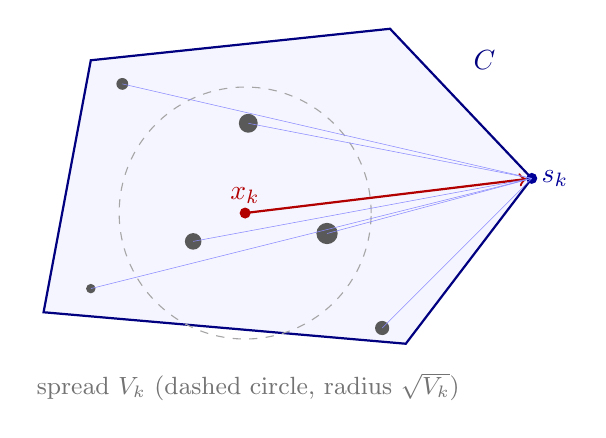
\begin{tikzpicture}[scale=1.0]
  \fill[blue!4] (0,0) -- (4.6,-0.4) -- (6.2,1.7) -- (4.4,3.6) -- (0.6,3.2) -- cycle;
  \draw[blue!50!black, thick] (0,0) -- (4.6,-0.4) -- (6.2,1.7) -- (4.4,3.6) -- (0.6,3.2) -- cycle;
  \node[blue!50!black] at (5.6,3.2) {$C$};
  \foreach \x/\y/\r in {0.6/0.3/0.06, 1.0/2.9/0.075, 4.3/-0.2/0.09, 1.9/0.9/0.105, 2.6/2.4/0.12, 3.6/1.0/0.135}
    \fill[black!65] (\x,\y) circle (\r);
  \coordinate (xk) at (2.56,1.26);
  \draw[black!35, dashed] (xk) circle (1.6);
  \fill[red!70!black] (xk) circle (0.07);
  \node[red!70!black, above] at (xk) {$x_k$};
  \coordinate (sk) at (6.2,1.7);
  \fill[blue!60!black] (sk) circle (0.07);
  \node[blue!60!black, right] at (sk) {$s_k$};
  \draw[->, thick, red!70!black, shorten >=2pt] (xk) -- (sk);
  \foreach \x/\y in {0.6/0.3, 1.0/2.9, 4.3/-0.2, 1.9/0.9, 2.6/2.4, 3.6/1.0}
    \draw[blue!45, very thin] (\x,\y) -- (sk);
  \node[black!55, align=center, font=\small] at (2.6,-0.95) {spread $V_k$ (dashed circle, radius $\sqrt{V_k}$)};
\end{tikzpicture}
\caption{The iterate $x_k$ is the center of mass of the earlier oracle points
(gray disks, sized by weight). Every gray point is within $D$ of $s_k$ (thin blue
lines), and the mean of their squared distances to $s_k$ equals
$\|s_k-x_k\|^2+V_k$. So the step $s_k-x_k$ (red) can have length close to $D$ only
if the cloud is tightly bunched, and each long step spreads the cloud.}
\label{fig:cloud}
\end{figure}

\subsection{Results}

\begin{theorem}\label{thm:main}
For every $N\ge1$, the iterates~\eqref{eq:fw} satisfy
\[
  f(x_N)-f^\star \;\le\; LD^2\,\frac{N+\frac13 H_{N-1}}{N(N+1)},\qquad
  H_m=\sum_{j=1}^m\frac1j,\quad H_0=0.
\]
\end{theorem}

\begin{corollary}\label{cor:simple}
For every $N\ge1$,
\[
  f(x_N)-f^\star\le\frac{LD^2}{N+1}\Bigl(1+\frac{H_{N-1}}{3N}\Bigr)\le\frac43\,\frac{LD^2}{N+1},
  \qquad
  \limsup_{N\to\infty}\frac{N\,(f(x_N)-f^\star)}{LD^2}\le1.
\]
\end{corollary}

In practical terms, the number of iterations that guarantees an error of at most
$\varepsilon LD^2$ drops from about $2/\varepsilon$ to about $1/\varepsilon$; for
$\varepsilon=1\%$, from $198$ to $101$. Nothing about the algorithm changes. What
changes is what we can promise about it.

The bound cannot be improved at $N=1$. Take $f(x)=\frac L2x^2$ on $C=[0,D]$ and
$x_0=0=x^\star$. Then $\nabla f(x_0)=0$, the oracle may return $s_0=D$, and
$f(x_1)-f^\star=LD^2/2$. For larger $N$ the bound is not exact.
Section~\ref{sec:numerics} compares it with the true worst case, computed by PEP:
the true constant appears to be about $0.9$, so Theorem~\ref{thm:main} removes
most of the slack in the classical bound but not all of it
(Figure~\ref{fig:constants}).

In practice one rarely knows $f^\star$, so solvers stop when the Frank--Wolfe gap,
a computable upper bound on the error, is small. Section~\ref{sec:gap} improves the
classical guarantee for this gap from $\frac{27}{4}LD^2/(N+2)$ to $3LD^2/(N+1)$.
Section~\ref{sec:proof} proves Theorem~\ref{thm:main}.

\section{Proof of Theorem~\ref{thm:main}}\label{sec:proof}

The proof has five steps. Step~1 is the classical one-step inequality. Step~2
tracks the spread of the cloud and turns the picture of Figure~\ref{fig:cloud} into
two exact relations. Step~3 handles the first step. Steps~4 and~5 combine the
relations through a potential function and solve the resulting recursion in
closed form.

By the scaling $x\mapsto x/D$, $f\mapsto f/(LD^2)$ we assume $L=D=1$. Write
$e_k=f(x_k)-f^\star$ for the error and $\delta_k=\|s_k-x_k\|^2$ for the squared
step length.

\paragraph{Step 1: descent.}
By smoothness on the segment $[x_k,x_{k+1}]\subset C$, by the definition of $s_k$,
and by convexity,
\[
  f(x_{k+1})\le f(x_k)+h_k\langle\nabla f(x_k),s_k-x_k\rangle+\tfrac{h_k^2}{2}\delta_k,
  \qquad
  \langle\nabla f(x_k),s_k-x_k\rangle\le\langle\nabla f(x_k),x^\star-x_k\rangle\le-e_k,
\]
so that
\begin{equation}\label{eq:descent}
  e_{k+1}\le(1-h_k)e_k+\tfrac{h_k^2}{2}\,\delta_k .
\end{equation}
The classical proof stops here and uses $\delta_k\le1$.

\paragraph{Step 2: the spread of the cloud.}
Define probability measures $\mu_0=\varepsilon_{x_0}$ and
$\mu_{k+1}=(1-h_k)\mu_k+h_k\,\varepsilon_{s_k}$, where $\varepsilon_y$ is the Dirac
mass at $y$. By induction, $\mu_k$ is supported on a finite subset of $C$ and has
mean $x_k$; for $k\ge1$ it is the cloud of~\eqref{eq:average}. Let
$V_k=\E_{Y\sim\mu_k}\|Y-x_k\|^2$. For any point $s$,
$\E\|s-Y\|^2=\|s-x_k\|^2+V_k$; taking $s=s_k\in C$ and using $\operatorname{diam}C=1$,
\begin{equation}\label{eq:delta}
  \delta_k=\E_{Y\sim\mu_k}\|s_k-Y\|^2-V_k\le1-V_k .
\end{equation}
This is the first relation: spread limits step length. For the second, note that
$x_{k+1}-x_k=h_k(s_k-x_k)$ and $s_k-x_{k+1}=(1-h_k)(s_k-x_k)$. The law of total
variance for the mixture $\mu_{k+1}$ gives
\begin{equation}\label{eq:variance}
  V_{k+1}=(1-h_k)\bigl(V_k+h_k^2\delta_k\bigr)+h_k(1-h_k)^2\delta_k
  =(1-h_k)V_k+h_k(1-h_k)\,\delta_k .
\end{equation}
This is the second relation: step length builds spread. It is convenient to work
with the room left, $W_k:=1-V_k$, in which~\eqref{eq:delta}--\eqref{eq:variance}
become
\begin{equation}\label{eq:room}
  0\le\delta_k\le W_k,\qquad
  W_{k+1}=h_k+(1-h_k)W_k-h_k(1-h_k)\,\delta_k .
\end{equation}
A long step (large $\delta_k$) uses up room, and room is what later steps need.

\paragraph{Step 3: the first step.}
Since $h_0=1$, we have $x_1=s_0$ and $\mu_1=\varepsilon_{s_0}$, hence $W_1=1$, and
\eqref{eq:descent} with~\eqref{eq:delta} ($V_0=0$) gives $e_1\le\frac12$. This is
the case $N=1$.

\paragraph{Step 4: a potential.}
Let $E_k=k(k+1)e_k$. Since $(k+1)(k+2)(1-h_k)=k(k+1)$ and
$(k+1)(k+2)h_k^2/2=2(k+1)/(k+2)$, inequality~\eqref{eq:descent} gives, for $k\ge1$,
\begin{equation}\label{eq:E}
  E_{k+1}\le E_k+\frac{2(k+1)}{k+2}\,\delta_k .
\end{equation}
A long step raises $E$ but uses up room $W$. We look for prices $\alpha_k\ge0$ that
make the potential $\Phi_k=E_k+\alpha_kW_k$ indifferent to the step length, so
that the two effects cancel. Fix $N\ge2$, set $\alpha_N=0$, and for
$k=N-1,\dots,1$ define
\begin{equation}\label{eq:alpha}
  \alpha_k=\frac{2(k+1)}{k+2}+\alpha_{k+1}\Bigl(\frac{k}{k+2}\Bigr)^2 .
\end{equation}

\begin{lemma}\label{lem:alpha}
$0\le\alpha_k\le k+1$ for $2\le k\le N$.
\end{lemma}

\begin{proof}
Nonnegativity is clear. Use backward induction from $\alpha_N=0$: if
$\alpha_{k+1}\le k+2$, then $\alpha_k\le2+k^2/(k+2)$, which is at most $k+1$ if and
only if $2k+4\le3k+2$, that is, $k\ge2$.
\end{proof}

By~\eqref{eq:E} and~\eqref{eq:room},
\[
  \Phi_{k+1}\le E_k+c_k\,\delta_k+\alpha_{k+1}\bigl(h_k+(1-h_k)W_k\bigr),\qquad
  c_k:=\frac{2(k+1)}{k+2}-\alpha_{k+1}h_k(1-h_k).
\]
Since $h_k(1-h_k)=2k/(k+2)^2$ and $\alpha_{k+1}\le k+2$ (Lemma~\ref{lem:alpha}, or
$\alpha_N=0$), we have $c_k\ge2/(k+2)>0$, so $\delta_k\le W_k$ yields
\[
  \Phi_{k+1}\le E_k+\alpha_{k+1}h_k+W_k\bigl(c_k+\alpha_{k+1}(1-h_k)\bigr)
  =\Phi_k+\alpha_{k+1}h_k,
\]
because $c_k+\alpha_{k+1}(1-h_k)=\frac{2(k+1)}{k+2}+\alpha_{k+1}(1-h_k)^2=\alpha_k$.
Summing over $k=1,\dots,N-1$, and using $\Phi_N=E_N$ and
$\Phi_1=E_1+\alpha_1W_1\le1+\alpha_1$ (Step~3),
\begin{equation}\label{eq:BN}
  E_N\le B_N:=1+\alpha_1+\sum_{k=1}^{N-1}\alpha_{k+1}h_k .
\end{equation}

\paragraph{Step 5: evaluating $B_N$.}
Rather than solve~\eqref{eq:alpha} directly, we evaluate $B_N$ on the path that
makes every inequality tight. Define numbers $\bar E_1=\bar W_1=1$ and
$\bar W_{k+1}=h_k+(1-h_k)^2\bar W_k$,
$\bar E_{k+1}=\bar E_k+\frac{2(k+1)}{k+2}\bar W_k$. These satisfy all relations of
Step~4 with equality (take $\delta_k=\bar W_k$), hence $\bar E_N=B_N$. By induction,
\[
  \bar W_k=\frac{(k+2)(3k+1)}{6k(k+1)},
\]
since
$\frac{2}{k+2}+\frac{k^2}{(k+2)^2}\cdot\frac{(k+2)(3k+1)}{6k(k+1)}
=\frac{3k^2+13k+12}{6(k+1)(k+2)}=\frac{(k+3)(3k+4)}{6(k+1)(k+2)}$.
Therefore $\frac{2(k+1)}{k+2}\bar W_k=\frac{3k+1}{3k}=1+\frac1{3k}$ and
\[
  B_N=\bar E_N=1+\sum_{k=1}^{N-1}\Bigl(1+\frac1{3k}\Bigr)=N+\tfrac13H_{N-1}.
\]
Combining with~\eqref{eq:BN}, $e_N=E_N/(N(N+1))\le(N+\frac13H_{N-1})/(N(N+1))$.
\qed

\begin{remark}[What the argument captures, and what it misses]\label{rem:captures}
Inequalities~\eqref{eq:descent}--\eqref{eq:variance} define a linear program in
$(\delta_k)$ whose value is exactly $B_N/(N(N+1))$. Its worst case saturates
$\delta_k=1-V_k$, so the spread of the cloud tends to $D^2/2$. In the exact PEP of
Frank--Wolfe, the improvement over $2LD^2/N$ comes almost entirely from the pairwise
diameter constraints among $\{x_0,s_0,s_1,\dots\}$. Dropping them restores a
leading constant close to $2$, while dropping the cross linear-minimization
constraints or the optimality constraints of $x^\star$ hardly changes the value.
The variance identity is a convenient aggregate of exactly those pairwise
constraints, which is why a single number can capture most of the improvement.
For the step sizes $h_k=\ell/(k+\ell)$ the same argument gives the smallest
asymptotic constant at $\ell=2$.
\end{remark}

\section{Consequence for the Frank--Wolfe gap}\label{sec:gap}

The error $f(x_k)-f^\star$ cannot be computed without knowing $f^\star$. The
Frank--Wolfe (duality) gap
\[
  g_k=\max_{s\in C}\langle\nabla f(x_k),x_k-s\rangle=\langle\nabla f(x_k),x_k-s_k\rangle
\]
can: the method computes $s_k$ anyway. By convexity $g_k\ge f(x_k)-f^\star$, so the
gap is the standard stopping certificate, and solvers stop once it falls below a
tolerance. A guarantee on the gap therefore bounds how long a solver runs. The
classical guarantee is
$\min_{k\le N}g_k\le\frac{27}{4}LD^2/(N+2)$~\cite[Thm.~2]{Jag13}.

\begin{corollary}\label{cor:gap}
For every $N\ge1$, $\displaystyle\min_{0\le k\le N}g_k\le\frac{3\,LD^2}{N+1}$.
\end{corollary}

\begin{proof}
Take $L=D=1$. Smoothness gives $h_kg_k\le e_k-e_{k+1}+h_k^2/2$. Summing over
$K_0\le k\le N$ and using $e_{N+1}\ge0$,
\[
  \Bigl(\min_{K_0\le k\le N}g_k\Bigr)\sum_{k=K_0}^Nh_k\;\le\;e_{K_0}+\tfrac12\sum_{k=K_0}^Nh_k^2,
\]
and we bound $e_{K_0}$ by Theorem~\ref{thm:main}.

For $N\le400$, optimizing over $K_0$ in exact rational arithmetic gives
$(N+1)\min_kg_k\le2.8984<3$. For $N>400$, take $m=K_0=\lceil N/2\rceil\ge200$. Then
\begin{itemize}
  \item $\frac12\sum_{k\ge m}h_k^2\le\frac2{m+1}-\frac2{N+2}$;
  \item $e_m\le\frac1{m+1}\bigl(1+\frac{1+\ln m}{3m}\bigr)\le\frac{1.0105}{m+1}$;
  \item $\frac1{m+1}\le\frac2{N+2}$.
\end{itemize}
So the right-hand side is at most $4.021/(N+2)$. Moreover
$\sum_{k=m}^Nh_k\ge2\ln\frac{N+3}{m+2}\ge2\ln\frac{2\cdot403}{405}\ge1.3763$. Hence
$\min_kg_k\le2.9217/(N+2)<3/(N+1)$.
\end{proof}

The asymptotic constant of this argument is
$\min_{\theta\in(0,1)}\frac{3/\theta-2}{2\ln(1/\theta)}\approx2.882$. If the
variance constraint is also used inside the sum (a linear program over
$e_k,g_k,\delta_k,V_k$), numerically $(N+2)\min_kg_k\to\approx2.15$, against
$\approx4.30$ for the classical relaxation $\delta_k\le D^2$. The PEP value is
$\approx1.67$.

\section{How close is the bound to the truth?}\label{sec:numerics}

We computed the exact worst-case value $w_N=\sup\,(f(x_N)-f^\star)/(LD^2)$ by solving
the tight PEP~\cite{THG17}. We used the interpolation conditions for $L$-smooth
convex functions together with $C=\operatorname{conv}\{x_0,s_0,\dots,s_{N-1},x^\star\}$
(linear-oracle optimality of each $s_k$, optimality of $x^\star$ with respect to all
vertices, and all pairwise vertex distances at most $D$), and solved with the
interior-point solver Clarabel. Table~\ref{tab:pep} lists the values and
Figure~\ref{fig:constants} plots the constants. These values are exact for
functions that are $L$-smooth on all of $\R^d$. Theorem~\ref{thm:main} needs
smoothness only on $C$; for that larger class the values are lower bounds on the
worst case.

\begin{table}[htbp]
\centering
\begin{tabular}{rcccc}
\toprule
$N$ & PEP $w_N$ & $Nw_N$ & Thm.~\ref{thm:main} & Jaggi $2/(N+2)$\\
\midrule
 1 & 0.50000 & 0.500 & 0.50000 & 0.66667\\
 2 & 0.31262 & 0.625 & 0.38889 & 0.50000\\
 3 & 0.22785 & 0.684 & 0.29167 & 0.40000\\
 5 & 0.14621 & 0.731 & 0.18981 & 0.28571\\
10 & 0.07829 & 0.783 & 0.09948 & 0.16667\\
20 & 0.04132 & 0.826 & 0.05043 & 0.09091\\
40 & 0.02156 & 0.863 & 0.02525 & 0.04762\\
60 & 0.01468 & 0.881 & 0.01682 & 0.03226\\
80 & 0.01116 & 0.893 & 0.01260 & 0.02439\\
\bottomrule
\end{tabular}
\caption{Exact worst case (PEP, numerical), the bound of Theorem~\ref{thm:main},
and the classical bound ($L=D=1$). At $N=3$ the PEP value agrees with $18/79$ to
eight digits. For $N=60$ and $N=80$ the solver reported reduced accuracy.}
\label{tab:pep}
\end{table}

\begin{figure}[htbp]
\centering
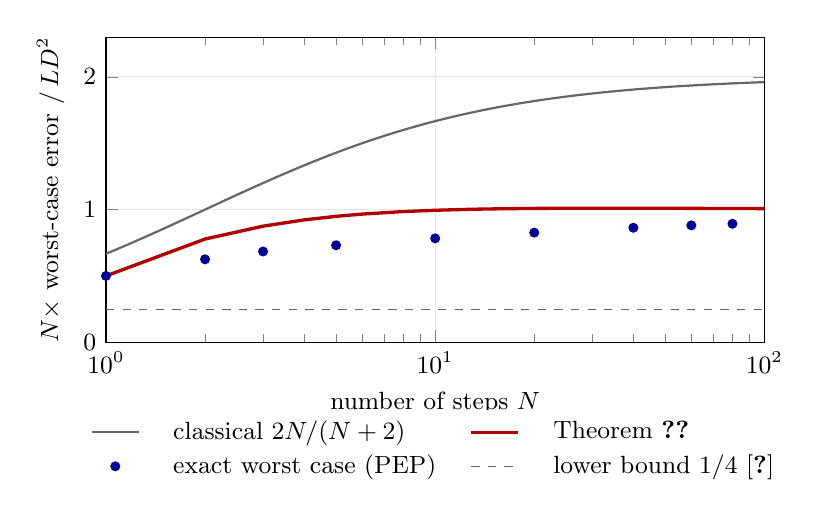
\begin{tikzpicture}
\begin{axis}[
  width=0.82\textwidth, height=0.45\textwidth,
  xmode=log, xmin=1, xmax=100, ymin=0, ymax=2.3,
  xlabel={number of steps $N$},
  ylabel={$N\times$ worst-case error $/\,LD^2$},
  legend cell align=left,
  legend style={font=\small, draw=none, at={(0.5,-0.22)}, anchor=north, legend columns=2, column sep=10pt},
  tick label style={font=\small}, label style={font=\small},
  grid=major, grid style={black!10}]
\addplot[black!60, thick, domain=1:100, samples=60] {2*x/(x+2)};
\addlegendentry{classical $2N/(N+2)$}
\addplot[red!70!black, very thick] coordinates {
(1,0.5000) (2,0.7778) (3,0.8750) (4,0.9222) (5,0.9491) (6,0.9659) (8,0.9849)
(10,0.9948) (13,1.0025) (16,1.0062) (20,1.0087) (25,1.0099) (30,1.0103)
(40,1.0102) (50,1.0097) (60,1.0091) (70,1.0085) (80,1.0080) (100,1.0072)};
\addlegendentry{Theorem~\ref{thm:main}}
\addplot[blue!60!black, only marks, mark=*, mark size=1.6pt] coordinates {
(1,0.500) (2,0.625) (3,0.684) (5,0.731) (10,0.783) (20,0.826) (40,0.863)
(60,0.881) (80,0.893)};
\addlegendentry{exact worst case (PEP)}
\addplot[black!60, dashed, domain=1:100, samples=2] {0.25};
\addlegendentry{lower bound $1/4$~\cite{Lan13}}
\end{axis}
\end{tikzpicture}
\caption{The constant in the Frank--Wolfe rate: $N$ times the worst-case error after
$N$ steps, in units of $LD^2$. The classical bound tends to $2$, Theorem~\ref{thm:main}
to $1$, and the exact worst case appears to approach about $0.9$. Lan's lower bound
holds for every linear-minimization method.}
\label{fig:constants}
\end{figure}

The sequence $Nw_N$ increases slowly, and extrapolation suggests a limit near
$0.9$--$0.95$. The exact constant $c^\star=\lim_NNw_N$ lies in $[1/4,1]$
by~\cite{Lan13} and Theorem~\ref{thm:main}. Determining it remains open.
Remark~\ref{rem:captures} suggests where to look. The variance identity sums the
pairwise distance constraints into one number; the gap between our constant $1$
and the PEP value of about $0.9$ presumably comes from using them one by one.

\section*{Reproducibility}
All computations are in the accompanying repository,
\url{https://github.com/samsonmaximus/Frank-Wolfe-Constant-Halved}, under
\path{experiments/} (Python~3.11, numpy, scipy, cvxpy
with Clarabel):
\begin{itemize}
  \item \texttt{pep\_fw.py}: the exact PEP, which produces the values $w_N$ of
  Table~\ref{tab:pep};
  \item \texttt{pep\_fw\_ablate.py}, \texttt{pep\_fw\_local.py}: the
  constraint-ablation experiments described in Remark~\ref{rem:captures};
  \item \texttt{variance\_lp.py}: the linear program defined
  by~\eqref{eq:descent}--\eqref{eq:variance}, for general $\ell$;
  \item \texttt{check\_proof.py}: exact rational checks of~\eqref{eq:alpha}, of
  Lemma~\ref{lem:alpha}, of $c_k>0$ and of $B_N=N+\frac13H_{N-1}$ (for $N\le199$
  and $N=500,1000$), and random feasible paths;
  \item \texttt{referee\_fw.py}: an independent check, which runs Frank--Wolfe on
  random and adversarial instances;
  \item \texttt{gap\_corollary\_all.py}: the exact rational check of
  Corollary~\ref{cor:gap} for every $N\le400$; \texttt{gap\_lp.py}: the variance
  relaxation for the gap.
\end{itemize}

\section*{Acknowledgements}
The proof was found and checked with the help of AI-assisted computational tools.
All arguments have been verified line by line, and the numerical claims can be
reproduced with the scripts above.

\begin{thebibliography}{9}
\bibitem{FW56} M.~Frank and P.~Wolfe. An algorithm for quadratic programming.
\emph{Naval Res.\ Logist.\ Quart.} 3 (1956) 95--110.
\bibitem{Jag13} M.~Jaggi. Revisiting Frank--Wolfe: projection-free sparse convex
optimization. ICML 2013.
\bibitem{FG16} R.~M.~Freund and P.~Grigas. New analysis and results for the
Frank--Wolfe method. \emph{Math.\ Program.} 155 (2016). arXiv:1307.0873.
\bibitem{BCC22} G.~Braun, A.~Carderera, C.~W.~Combettes, H.~Hassani, A.~Karbasi,
A.~Mokhtari, S.~Pokutta. Conditional gradient methods. arXiv:2211.14103.
\bibitem{Bac15} F.~Bach. Duality between subgradient and conditional gradient
methods. \emph{SIAM J.\ Optim.} 25 (2015). arXiv:1211.6302.
\bibitem{Nes18} Yu.~Nesterov. Complexity bounds for primal-dual methods minimizing
the model of objective function. \emph{Math.\ Program.} 171 (2018).
\bibitem{Lan13} G.~Lan. The complexity of large-scale convex programming under a
linear optimization oracle. arXiv:1309.5550.
\bibitem{THG17} A.~B.~Taylor, J.~M.~Hendrickx, F.~Glineur. Exact worst-case
performance of first-order methods for composite convex optimization. \emph{SIAM J.\
Optim.} 27 (2017). arXiv:1512.07516.
\bibitem{LG24} A.~Luner and B.~Grimmer. Performance estimation for smooth and
strongly convex sets. arXiv:2410.14811.
\end{thebibliography}

\end{document}
